\chapter{Исследовательский раздел}\label{ch:ch1}
\section{Процесс сертификации ПО на отсутствие НДВ}\label{sec:ch1/sec1}
Сертификация программного обеспечения проводится, 
когда необходимо подтвердить соответствие разрабатываемой 
продукции требованиям защиты информации.

Сертификационная процедура состоит из следующих этапов:
\begin{enumerate}
    \item Готовность документации ПО, доступность исходных текстов
    \item Опредление объема исходных текстов, подлежащих анализу
    \item Обращение заявителя в испытательную лабораторию с собранной информацией
    \item Анализ документации
    \item Разработка <<Программы и методик проведения сертификационных испытаний>>
    \item Проведение испытаний
    \item Экспертиза результатов
\end{enumerate}

Сертификация должна выявить присутствие в исполняемом файле недекларированных возможностей,
которые могут являться как злым умыслом\autocite{compile-a-virus, ken-thompson-hack} 
разработчиков компилятора, линкера и других вспомогательных программ,
так и методами оптимизации ПО, которые применяются для более рационального 
потребления ресурсов программой.

Выявить данные расхождения между необработанными исходными кодами и 
поведением программы во время исполнения позволяет разработанный мной
программный модуль.

Дадим определение термину <<Недекларированные возможности>>:

\textbf{Недекларированные возможности}\autocite{undeclared-capabilities-antimalware} 
— намеренно измененная часть ПО, с помощью которой можно получить незаметный 
несанкционированный доступ к безопасной компьютерной среде.

\section{Классификация НДВ}\label{sec:ch1/sec2}
    \subsection{По применению}\label{sec:ch1/sec2/sub1}
    \begin{itemize}
        \item \textbf{Перехват данных}
        \item \textbf{Подмена данных}
        \item \textbf{Вывод компьютерной системы из строя}
        \item \textbf{Полный доступ к удаленной компьютерной системе}

              Такие программы могут быть использованы злоумышленниками для
              всех вышеперечисленных целей
    \end{itemize}
\subsection{По целям}\label{sec:ch1/sec2/sub2}
\begin{itemize}
    \item \textbf{Персональные компьютеры и рабочие станции}
          
          Целью могут быть как персональные компьютеры широкого числа пользователей,
          так и отдельные рабочие станции, которые могут являться точкой входа в
          защищенную компьютерную систему, так и использоваться для перехвата важной
          информации
    \item \textbf{Серверы}
          
          Серверы обслуживают большое количество клиентов, а значит проникновение на
          сервер может существенно повлиять на работу всех компьютеров, работающих с
          данным сервером
    \item \textbf{Встраиваемые системы}

          Благодаря постоянному удешелению микроконтроллеров и периферийных устройств,
          все больше и больше повседневных вещей обзаводятся <<умной>> функциональностью.
          Погоня производителей за прибылями отражается на безопасности прошивок умных устройств.
    \item \textbf{Промышленные компьютеры}

        Программные закладки в такие системы чреваты шпионажем или диверсией\autocite{stuxnet}
        \footnote{Хотя данная программа является вирусом, а не программой с НДВ, случившееся
        ярко показывает реальное применение подобных техник для деструктивных действий}.
\end{itemize}

\section{Степень опасности НДВ}\label{sec:ch1/sec3}
Для определения опасности НДВ будем пользоваться следующими нормативными документами:
\begin{itemize}
    \item Приказ ФСТЭК России от 18 февраля 2013 г. № 21
    \item Федеральный закон "О персональных данных" от 27.07.2006 N 152-ФЗ
\end{itemize}

Тип угроз безопасности персональных данных определяется 
в зависимости от комбинаций критичности угроз в ИСПДн (\autoref{table:threats}):
\begin{itemize}
    \item Наличием НДВ в системном программном обеспечении (ПО), используемом в ИСПДн
    \item Наличием НДВ в прикладном ПО, используемом в ИСПДн
\end{itemize}



\begin{table}[!htbp]
    \centering
    \caption{\label{table:threats}Тип актуальных угроз}


    \begin{center}
        \begin{tabular}{ | c | c | c | c | }
            \hline
            Угрозы & \multicolumn{3}{ c |}{Тип актуальных угроз} \\
            \cline{2-4}
                   & 1 Тип & 2 Тип & 3 Тип\\
            \hline
            \makecell{Наличие НДВ в системном ПО,\\ используемом в ИСПДн} & \redcell{критично} & \greencell{некритично} & \redcell{некритично} \\
            \hline
            \makecell{Наличие НДВ в прикладном ПО \\ используемом в ИСПДн} & \makecell{критично \\ или \\ некритично} & \redcell{критично} & \greencell{некритично} \\
            \hline
        \end{tabular}
    \end{center}


\end{table}

Порядок определения актуальных угроз безопасности 
персональных данных в ИСПДн осуществляется 
в соответствии с Методикой определения 
актуальных угроз безопасности персональных данных 
при их обработке в информационных 
системах персональных данных, утвержденных 
ФСТЭК России, 2008 год.

Актуальной считается угроза, которая может быть 
реализована в ИСПДн и представляет опасность для 
персональных данных.  Подход к составлению перечня 
актуальных угроз состоит в следующем. 
Для оценки возможности реализации угрозы применяются два показателя: 

$Y_1$ - уровень исходной защищенности ИСПДн\\
$Y_2$ - частота (вероятность) реализации рассматриваемой угрозы.\\
Коэффициент реализуемости угрозы $Y$ определяется соотношением: 

\[Y = \frac{Y_1 + Y_2}{20}\]

По значению коэффициента реализуемости угрозы Y 
интерпретация реализуемости угрозы следующим образом: 
\begin{itemize}
    \item если $0 \leq Y \leq 0.3$, то возможность реализации угрозы признается низкой
    \item если $0.3 < Y \leq  0.6$, то возможность реализации угрозы признается средней 
    \item если $0.6 < Y \leq  0.8$, то возможность реализации угрозы признается высокой 
    \item если $Y > 0,8$, то возможность реализации угрозы признается очень высокой
\end{itemize}

Далее оценивается опасность каждой угрозы.
Этот показатель имеет три значения: 
\begin{itemize}
    \item низкая опасность – если реализация угрозы может привести к незначительным негативным последствиям для субъектов персональных данных
    \item средняя опасность – если реализация угрозы может привести к негативным последствиям для субъектов персональных данных
    \item высокая опасность – если реализация угрозы может привести к значительным негативным последствиям для субъектов персональных данных.
\end{itemize}

Затем осуществляется выбор из общего
перечня угроз безопасности тех, 
которые относятся к актуальным для данной ИСПДн,
в соответствии с правилами, приведенными в \autoref{table:actual-threats}
\begin{table}[!htbp]
    \centering
    %\captionsetup{justification=centering}
    \caption{\label{table:actual-threats}Правила отнесения угрозы безопасности персональных данных к критичной}

    \begin{center}
        \begin{tabular}{ | c | c | c | c | }
            \hline
            \makecell{Возможность \\ реализации угрозы} & \multicolumn{3}{ c |}{Показатель опасности угрозы} \\
            \cline{2-4}
                   & Низкая & Средняя & Высокая\\
            \hline
            \makecell{Низкая}        & \greencell{некритичная} & \greencell{некритичная} & \redcell{критичная} \\
            \hline
            \makecell{Средняя}       & \greencell{некритичная} & \redcell{критичная}      & \redcell{критичная} \\
            \hline
            \makecell{Высокая}       & \redcell{критичная}      & \redcell{критичная}      & \redcell{критичная} \\
            \hline
            \makecell{Очень высокая} & \redcell{критичная}      & \redcell{критичная}      & \redcell{критичная} \\
            \hline
        \end{tabular}
    \end{center}


\end{table}

После чего выносится решение о проведении анализа ПО 
на НДВ в процесс сертификации или его игнорирование,
как некритичного.

\section{Обзор программных решений для сертификации ПО на отсутствие НДВ}\label{sec:ch1/sec3}
На сегодняшний день не существует в комплексных разработок по сертификации программного обеспечения
на предмет НДВ. Однако, существуют программы, специализирующиеся отдельно на анализе исходных кодов
и отдельно исполняемого файла. Так как {\ProgModule} будет совмещать и расширять функционал
данных программных средств, то рассмотрим их по отдельности.

\newpage
\subsection{Сравнение статических анализаторов}\label{sec:ch1/sec3/sub1}
\begin{table}[!htbp]
    {\small
        \setlength{\tabcolsep}{2pt}
        \caption{\label{table:static-analyzers-comparsion}
               Сравнительная таблица статических анализаторов}
        \begin{longtable}{*{4}{| c}|}
            \hline
            \diagbox[width=8cm]{Свойства}{Название программы}                                       &
            \makecell{Microsoft\\Application\\Inspector \autocite{microsoft-application-inspector}} &
            \makecell{SCI\\Tools\\Understand \autocite{sci-tools-understand}}                       &
            \makecell{GNU cflow \autocite{gnu-cflow}} \\
            \hline
            \makecell{Кросс-платформенность}             & \greencell{Да} & \greencell{Да} & \greencell{Да}\\
            \hline
            \makecell{Открытость\\исходного кода}        & \greencell{Да} & \redcell{Нет}   & \greencell{Да}\\
            \hline
            \makecell{Препроцессирование\\кода C/C++}    & \redcell{Нет}   & \greencell{Да} & \greencell{Да}\\
            \hline
            \makecell{Представление\\
                      препроцессорных директив как\\
                      вызов функций}                     & \redcell{Нет}   & \redcell{Нет}   & \greencell{Да}\\
            \hline
            \makecell{Создание графа вызовов}            & \redcell{Нет}   & \greencell{Да} & \greencell{Да} \\
            \hline
            \makecell{Создание обратного\\графа вызовов} & \redcell{Нет}   & \greencell{Да} & \greencell{Да}\\
            \hline
            \makecell{Бесплатность}                      & \greencell{Да} & \redcell{Нет}   & \greencell{Да}\\
            \hline
            \makecell{Графический интерфейс}             & Нет & Есть & Нет \\
            \hline
        \end{longtable}
    }
\end{table}

\subsubsection{Microsoft Application Inspector}\label{sec:ch1/sec3/sub1/sub1}

\begin{figure}[!htbp]
    \centerfloat{
        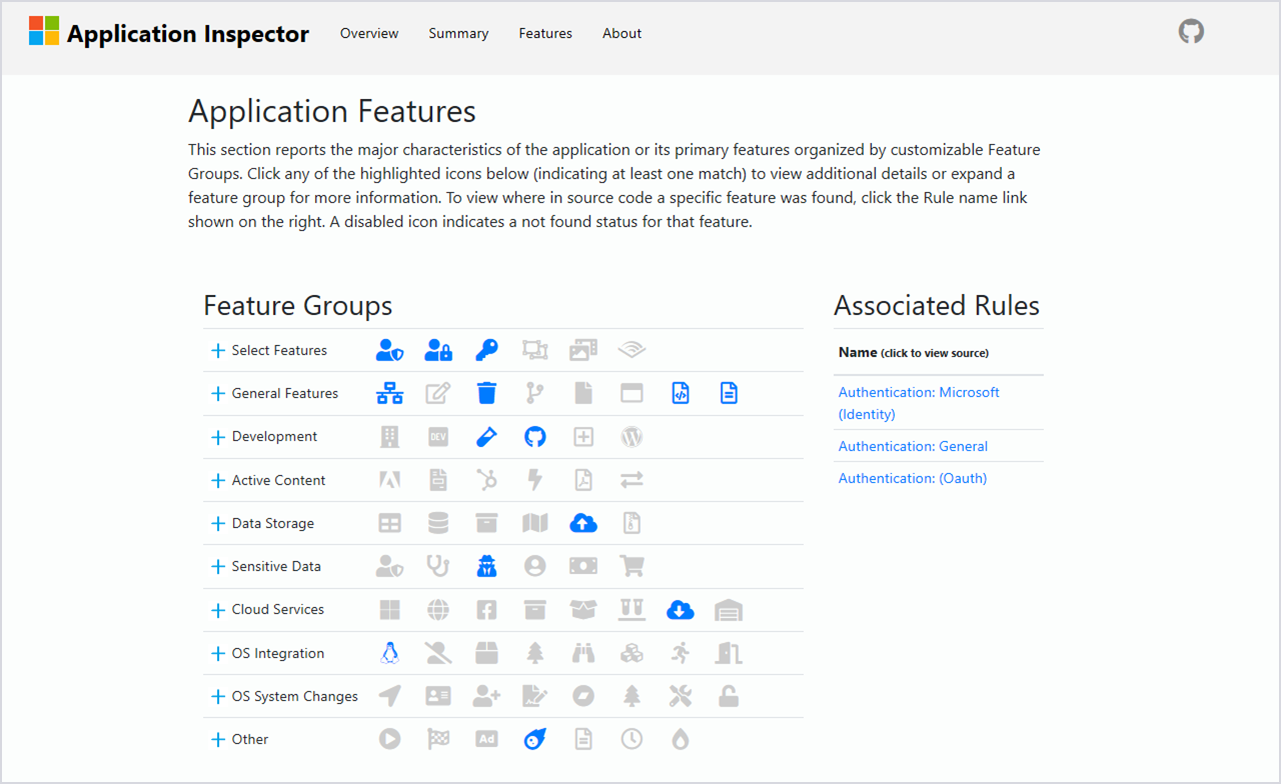
\includegraphics[width=\linewidth]{images/MSAppInspector.png}
    }
    \caption{Отчет Microsoft Application Inspector\label{fig:ms-app-inspector}}
\end{figure}
Задача Microsoft Application Inspector -- Систематическая и масштабируемая идентификация функций исходного кода.
Анализатор написан на .NET Core \autocite{net-core}, а это значит, что программа будет работать на всех платформах,
для которых реализован .NET Core: Windows, Linux и macOS.

Распознает паттерны не только в 34 языках, но так же и в их смешениях -- когда взаимодействующие части программы
написаны на разных языках. Является бесплатным ПО, с открытым исходным кодом.
В качестве недостатков для использования можно отметить предметный анализ функций, который ничего не говорит 
о последовательности их вызова.

\subsubsection{SCI Tools Understand}\label{sec:ch1/sec3/sub1/sub2}
SCI Tools Understand -- кросс-платформенный, быстрый статический анализатор больших объемов кода,
имеющий хорошие возможности в визуализации отношений модулей программы,
имеет встроенный расчет различных метрик программного кода.

Поддерживает около 20 языков программирования, а так же распознает различные их редакции.
Недостатки SCI Tools Understand -- платность и закрытый исходный код. Но купив лицензионную копию
программы, пользователь получает возможность писать скрипты манипуляции БД анализируемого проекта, 
генерирования отчетов и собственных метрик, 

\subsubsection{GNU cflow}\label{sec:ch1/sec3/sub1/sub3}
 Быстрый и минималистичный статический анализатор, с открытым исходным кодом,
 позволяющий создавать как прямые, так и обратные графы вызовов. 
 Командный интерфейс приближен к командному интерфейсу компилятора.
 Поддерживает языки C и C++, а так же LEX и YACC.
 К достоинствам так же можно отнести удобный и емкий формат отчета, который легко
 разбирать регулярными выражениями.

\subsubsection{Вывод}\label{sec:ch1/sec3/sub1/sub4}
Так как {\ProgModule} ориентирован на анализ C/C++ программ, то проанализировав
\autoref{table:static-analyzers-comparsion} приходим к выводу, что функционал 
Microsoft Application Inspector не покрывает нужные сценарии использования, 
а SCI Tools Understand  не подходит из-за своей закрытости и платности.
Единственный возможнный выбор -- GNU cflow. 

\subsection{Сравнение динамических анализаторов}\label{sec:ch1/sec3/sub2}
\begin{table}[!htbp]
    {\small
        \setlength{\tabcolsep}{2pt}
        \caption{\label{table:dynamic-analyzers-comparsion}
               Сравнительная таблица программ для динамического анализа}
        \begin{longtable}{*{3}{| c}|}
            \hline
            \diagbox[width=8cm]{Свойства}{Название программы} &
            \makecell{GDB \autocite{gdb}}                     &
            \makecell{QEMU \autocite{qemu}}                   \\
            \hline
            \makecell{Кросс-платформенность}             & \greencell{Да} & \greencell{Да} \\
            \hline
            \makecell{Открытость\\исходного кода}        & \greencell{Да} & \greencell{Да} \\
            \hline
            \makecell{Возможность\\анализировать память} & \greencell{Да} & \greencell{Да} \\
            \hline
            \makecell{Возможность\\программно управлять} & \greencell{Да} & \greencell{Да} \\
            \hline
            \makecell{Возможность\\создавать\\
                      собственные команды}               & \greencell{Да} & \redcell{Нет}   \\
            \hline
            \makecell{Возможность удаленной\\
                      отладки}                           & \greencell{Да} & \redcell{Нет}   \\
            \hline
            \makecell{Бесплатность}                      & \greencell{Да} & \greencell{Да} \\
            \hline
            \makecell{Графический интерфейс}             & Есть & Есть \\
            \hline
        \end{longtable}
    }
\end{table}

\subsubsection{GNU Debugger}\label{sec:ch1/sec3/sub2/sub1}
Отладчик GDB впервые увидел свет в 1986 году и за прошедшие годы обзавелся
большим количеством поддерживаемых архитектур процессоров, самые известные:
\begin{itemize}
    \item Alpha;
    \item ARM;
    \item AVR;
    \item H8/300;
    \item Altera Nios/Nios II;
    \item System/370;
    \item System 390;
    \item X86 и X86-64;
    \item IA-64 "Itanium";
    \item Motorola 68000;
    \item MIPS;
    \item PA-RISC;
    \item PowerPC;
    \item SuperH;
    \item SPARC;
    \item VAX;
\end{itemize}
К достоинствам можно отнести возможность описания сценария отладки в командном файле,
с последующим исполнением его GDB, а так же удаленную отладку.
\begin{figure}[!htbp]
    \centerfloat{
        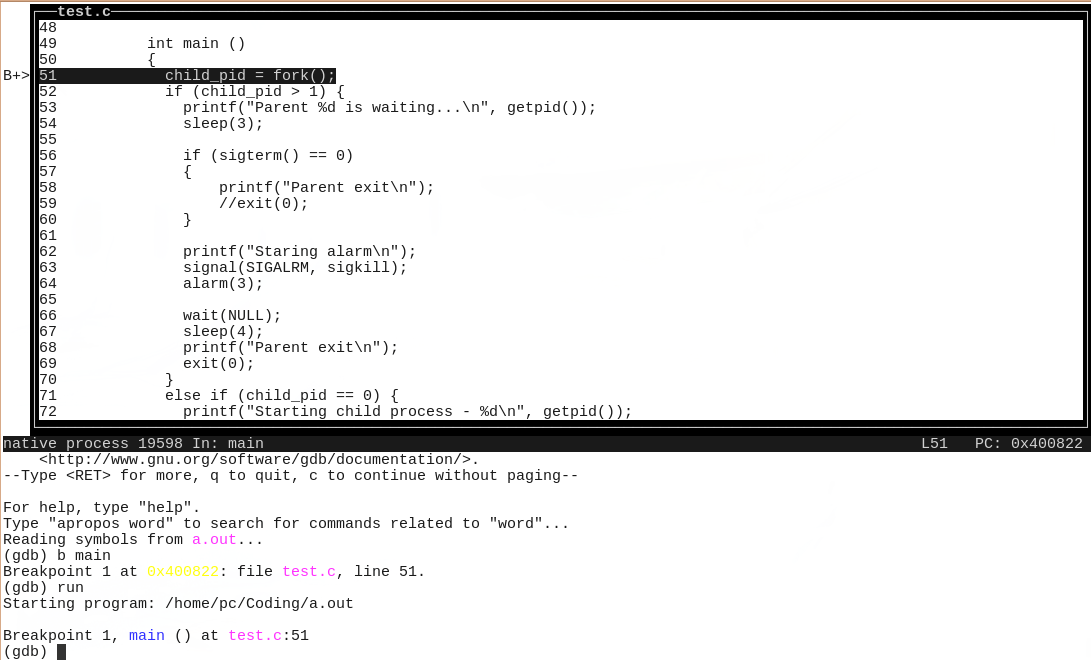
\includegraphics[width=\linewidth]{images/GDB.png}
    }
    \caption{Терминальный интерфейс GDB \label{fig:gdb-tui}}
\end{figure}

\subsubsection{QEMU}\label{sec:ch1/sec3/sub2/sub2}
\begin{figure}[!htbp]
    \centerfloat{
        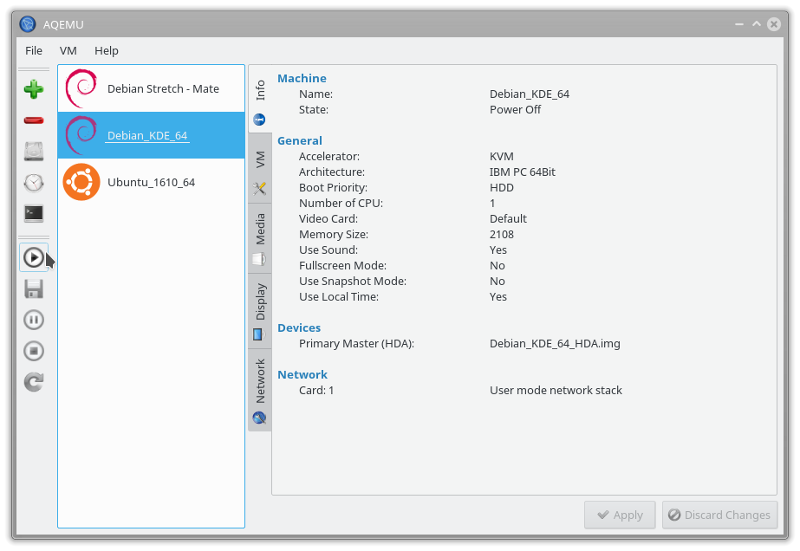
\includegraphics[width=\linewidth]{images/QEMU_GUI.png}
    }
    \caption{Графическая оболочка AQEMU для эмулятора QEMU\label{fig:aqemu}}
\end{figure}
QEMU -- Быстрый эмулятор процессоров, поддерживает множество просессорных архитектур,
предоставляет возможность сохранять сгенерированный машинный код.
К недостаткам можно отнести медленную, по сравнению с отладчиком работу,
так как эмулятору приходится преобразовывать каждую инструкцию запущенной программы
в машинный код процессора, на котором он запущен.

\subsubsection{Вывод}\label{sec:ch1/sec3/sub2/sub3}

Так как для более точного выполнения задачи сертификации будет полезно получать
информацию времени выполнения программы, такую, как:
\begin{enumerate}
    \item значения регистров перед вызовом функции;
    \item состояние стека перед вызовом функции;
    \item стек вызовов;
    \item экспертиза результатов;
    \item информацию о сегментах и функциях в них определенных;
\end{enumerate}
А так же расширять возможность динамического анализатора с помощью скриптов,
то из \autoref{table:dynamic-analyzers-comparsion} следует, что
удобнее всего это можно будет сделать с помощью отладчика GDB \autocite{gdb},
нежели эмулятора QEMU \autocite{qemu}.


\section{Постановка задачи ВКР}\label{sec:ch1/sec4}
На основе изложенного в \autoref{sec:ch1/sec1}-\autoref{sec:ch1/sec3} сформированы
следующие цели и задачи ВКР.
Цель: сокращение времени проведения сертификации программного обеспечения, написанного
на языках C и C++, а так же увеличение точности и подробности отчетов.

Задачи:
\begin{enumerate}
    \item исследование предметной области (рассмотрено в \autoref{sec:ch1/sec1});
    \item сравнительный анализ существующих программных решений 
        (рассмотрено в \autoref{sec:ch1/sec3/sub1}-\autoref{sec:ch1/sec3/sub2});
    \item выбор языка и среды разработки;
    \item разработка схемы данных {\ProgModule};
    \item разработка схемы алгоритма {\ProgModule};
    \item программирование {\ProgModule};
    \item отладка и тестирование {\ProgModule};
    \item разработка документации к {\ProgModule};
\end{enumerate}

\section{Выводы по разделу}\label{sec:ch1/sec5}
В исследовательском разделе обоснована актуальность разработки {\ProgModule}.
Исследована предметная область и проведен анализ возможных решений, из которых был сделан
вывод о том, что программы, аналогичной по функционалу {\ProgModule} нет на рынке.
Так же поставлены задачи для дальнейшей разработки {\ProgModule}.
